% !TEX root = thesis.tex

\section{Algunes definicions i els objectius de la teoria de nusos}\label{sec:Algunes definicions i els objectius de la teoria de nusos}

De definicions de nus, parlant en termes matemàtics, n'hi ha diverses. Nosaltres considerarem la definició dins el camp de la topologia, d'on en reutilitzarem molta notació. A més, la teoria de nusos s'emmarca dins una teoria més general; la de links. Per tant, moltes vegades anirem mencionant resultats que també son vàlids per aquests objectes. La següent secció pretén donar unes primeres definicions pel que fa als nostres objectes d'estudi.

\begin{definition}\label{def: Definició de nus}
	Diem que $L$ és un \underline{link} de m components, o un m-link si és un subconjunt de $S^3$, o de $\mathbb{R}^3$, que consisteix en m corbes disjuntes, simples, tancades i lineals a trossos. Un 1-link és un \underline{nus}.
\end{definition}

La condició de lineal a trossos significa que les components de $L$ estan cadascuna d'elles feta d'un nombre finit de rectes col·locades una al costat de l'altra amb el principi d'una coincidint amb el final de l'altra. Aquesta condició evita la creació de nusos patològics que no presenten un comportament esperat. A aquests últims nusos se'ls anomena \textit{salvatges} i no seran estudiats en aquest treball. A la pràctica, quan representem nusos o links assumirem que hi ha tants segments rectes que cada component semblarà corba.\\

\begin{figure}
	\centering
	\includegraphics[width=0.9\linewidth]{img/wildknot.png}
	\caption{Exemple d'un nus salvatge.}\label{fig:nussalvatge}
\end{figure}

\textit{De què tracta la teoria de nusos?}
Una possible resposta és que la teoria de nusos pretén classificar el conjunt de possibles nusos. Donat un nus $K$, hom considera que aquest està inclòs, mitjançant una aplicació contínua, dins l'espai ambient tres dimensional $\mathbb{R}^3$ o equivalentment dins $S^3$, obtenim aleshores la teoria clàssica de nusos. Aquesta teoria pretén estudiar la col·locació de $K$ dins aquest espai. Classificar, en aquest cas vol dir considerar iguals sota certes condicions, que definirem més endavant.

\begin{figure}
	\centering
	\includegraphics[width=0.45\linewidth]{img/7_1.jpg}
	\includegraphics[width=0.45\linewidth]{img/anell borromeu.jpg}
	\caption{A l'esquerra el nus $7_1$ (més endavant explicarem el perquè del nom). A la dreta un 3-link conegut amb el nom d'anell Borromeu. 
	}\label{fig:exemplesdenusosenmatematiques}
\end{figure}

\begin{definition}
	Diem que un nus està \underline{desnuat} o que és el nus trivial, notacionalment $\ovoid$ si no presenta cap creuament en els segments de corda que el formen.
\end{definition}

\subsection{Equivalència entre nusos}\label{Equivalència entre nusos}

Expliquem ara què entem quan diem que dos nusos son el mateix.

\begin{definition}\label{def: Definició d'isotopia ambient}
	Diem que dos links $L$ i $L'$ a $S^3$ son equivalents si existeix una isotopia ambient entre ells.
\end{definition}
És a dir, si existeix una família d'homeomorfismes $h_t:S^3\rightarrow S^3$ per $t\in[0, 1]$ tal que $h_0=1$, $h_1=h$ i $(x, t)\mapsto(h_{t}x, t)$ és un homeomorfisme lineal a trossos de $S^3\times[0, 1]$ a $S^3$, llavors direm que $L$ i $L'$ son links equivalents. L'equivalència entre nusos és la mateixa que en la Definició \ref{def: Definició d'isotopia ambient} tenint present que en aquest cas només tenim una component. Observem que la distorsió no és del mateix link sinó de l'espai "ambient" $S^3$ en sí mateix. Definir nus equivalent d'aquesta manera evita que els creuaments que formen el nus o link puguin fer-se cada vegada més petits fins a desapareixer. D'aquesta manera, és possible moure tot $S^3$ de forma contïnua utilitzant $h_t$ per passar de $L$ a $L'$.

\subsection{Representació d'un nus en matemàtiques}\label{sec:Representació de nus}
Tenint present la definició de nus a partir d'ara en sentit matemàtic donada a la Definició \ref{def: Definició de nus}, un pot veure la dificultat d'estudiar aquest tipus d'objectes tres dimensionals en un llibre de text o bé en una pissarra. És per això, que per tal d'estudiar-los sovint es representen els nusos mitjançant el seu \textit{diagrama de nus}.\\

Considerant la projecció paral·lela (o axonomètrica) sobre l'eix $z$ en el pla $\mathbb{R}^2$ d'un nus qualsevol $K$, obtindrem una figura com en l'exemple \ref{fig:projecció d'un nus sobre R2}.\\

\begin{figure}
	\centering
		\resizebox{7.5cm}{!}{
			
			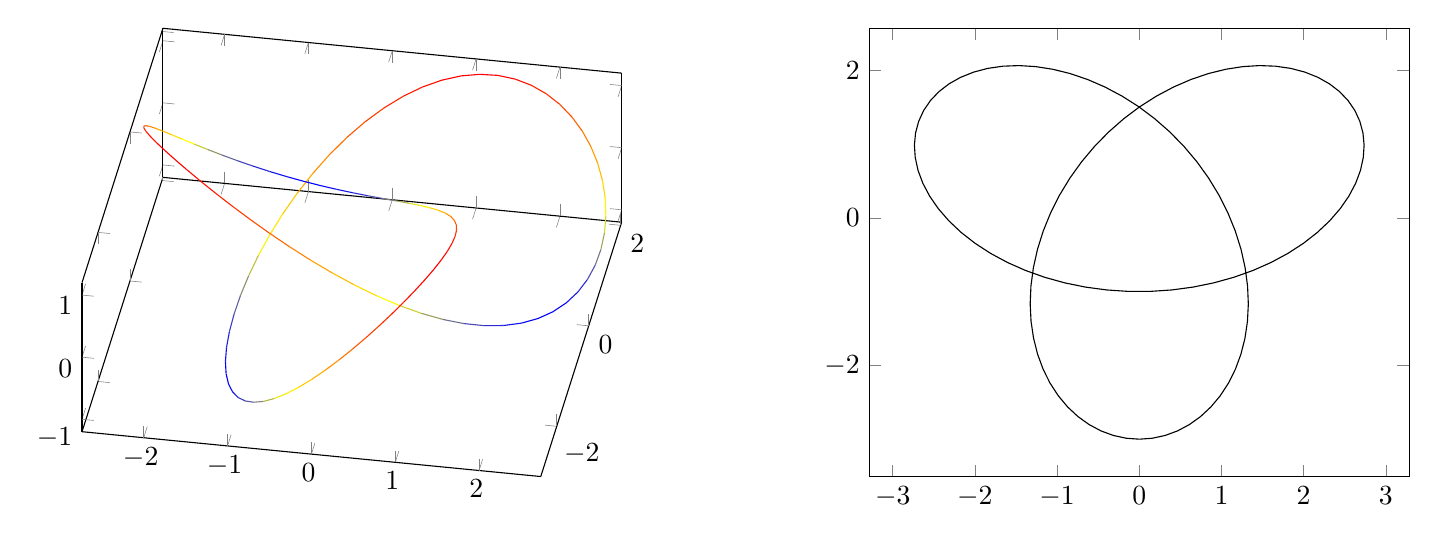
\begin{tikzpicture}
				
				\begin{scope}
					\begin{axis}
						\addplot [domain=-pi:pi,samples=120]({sin(deg(x))+2*sin(2*deg(x))},{cos(deg(x))-2*cos(2*deg(x))}); 
					\end{axis}
				\end{scope}
				
				\begin{scope}[xshift=-10cm]
					\begin{axis}
						[
						view={10}{60},
						]
						\addplot3[
						domain=-pi:pi,
						samples = 120,
						samples y=0,
						mesh
						]
						({sin(deg(x))+2*sin(2*deg(x))},
						{cos(deg(x))-2*cos(2*deg(x))},
						{-1*sin(3*deg(x))});
					\end{axis}
				\end{scope}
				
			\end{tikzpicture}
			
		}
	\caption{A l'esquerra el nus $3_1$ també conegut com Trefoil amb parametrització $(\sin t+2\sin 2t, \cos t-2\cos 2t,-\sin 3t)$. A la dreta, la seva projecció paral·lela sobre l'eix $z$.}\label{fig:projecció d'un nus sobre R2}
\end{figure}

Considerant aquesta projecció però, un perd informació sobre el propi nus, ja que cal saber quin segment de corda va per sobre i quin per sota alhora de creuar-se. Per tal de no perdre aquesta informació, el segment que passa per sota se'l dibuixa de forma discontínua mentre aquest passa sota el segment de corda que el creua.\\

\noindent
D'aquesta manera, la projecció del nus $3_1$ de la Figura \ref{fig:projecció d'un nus sobre R2} quedaria de la següent manera:

\begin{figure}[H]
	\resizebox{6.5cm}{!}{
		\begin{tikzpicture}[line width=0.5mm]
			\begin{scope}[rotate=270]
				\begin{knot}[
					consider self intersections=true,
					%  draft mode=crossings,
					flip crossing=2,
					only when rendering/.style={
						%    show curve controls
					}
					]
					\strand (0,2) .. controls +(2.2,0) and +(120:-2.2) .. (210:2) .. controls +(120:2.2) and +(60:2.2) .. (-30:2) .. controls +(60:-2.2) and +(-2.2,0) .. (0,2);
				\end{knot}
			\end{scope}
			
			\begin{scope}[xshift=-5cm, rotate=270]
				\begin{knot}[
					consider self intersections=false,
					%  draft mode=crossings,
					flip crossing=2,
					only when rendering/.style={
						%    show curve controls
					}
					]
					\strand (0,2) .. controls +(2.2,0) and +(120:-2.2) .. (210:2) .. controls +(120:2.2) and +(60:2.2) .. (-30:2) .. controls +(60:-2.2) and +(-2.2,0) .. (0,2);
				\end{knot}
			\end{scope}
		\end{tikzpicture}
	}
\end{figure}

Així doncs, considerant la projecció paral·lela sobre l'eix $z$ d'un nus $K$ qualsevol i disposant de la informació sobre els creuaments obtenim el que anomenarem \textit{diagrama de nus}, notacionalment $diag(K)$. Moltes vegades, en la literatura es fa un abús de llenguatge i notació, anomenant nus al que nosaltres anomenem diagrama de nus i fent servir $K$ i $diag(K)$ indistintament. D'aquí a no massa veurem que de fet, estudiar-ne les propietats d'un és equivalent a estudiar les de l'altre.\\